%实验报告-分光计1312

%文档类型
\documentclass[a4paper]{article}%A4纸,文档类型为论文

%宏包
%文字设置
\usepackage[UTF8]{ctex}%处理中文
\usepackage{xeCJK}%处理中文
\usepackage{fontspec,xunicode,xltxtra}%字体设置
%文档&排版设置
\usepackage{titlesec}%自定义章节标题样式
\usepackage{multicol}%分栏
\usepackage{hyperref}%超链接设置\daleth 
\usepackage{multirow,makecell}%制作复杂表格
\usepackage{booktabs}%画三线表要用
\usepackage{float}%图片、表格等位置浮动排版
\usepackage{indentfirst}%首行缩进
\usepackage{graphicx,subfigure}%图片插入
\usepackage{listings}%代码高亮
\usepackage{xcolor}
\usepackage{appendix}%附录
\usepackage{fancyhdr}%页眉页脚
\usepackage{geometry}%页边距
\usepackage{caption}
%数学
\usepackage{amsmath,amssymb}%公式
\usepackage{amsfonts,mathrsfs,txfonts}%数学字体
\usepackage{array}%矩阵
\usepackage{gensymb}%角度单位“度”的命令:\degree

\geometry{a4paper,scale=0.8}%设置了纸张为a4,并且版心占页面长度的比例为80%;scale也可以改为ratio,表示版面边距占页面长度的比例.~
\hypersetup{colorlinks=true,linkcolor=black,citecolor=black}%去掉目录等超链接所带的红框,并让参考文献的引用颜色为黑色
\setlength{\parindent}{2em}%首行缩进2字符
\lstset{
    columns=fixed,
    numbers=left, % 在左侧显示行号
    numberstyle=\footnotesize\color{darkgray},% 设定行号格式
    backgroundcolor=\color[RGB]{245,245,244},% 设定背景颜色
    keywordstyle=\color[RGB]{40,40,255},% 设定关键字颜色
    numberstyle=\color[RGB]{0,192,192},%行号数字样式
    commentstyle=\it\color[RGB]{0,96,96},% 设置代码注释的格式
    stringstyle=\rmfamily\slshape\color[RGB]{128,0,0},% 设置字符串格式
}
\pagestyle{fancy}%页眉页脚
\fancyhead{}%清空页眉
\fancyhead[C]{\emph{实验报告:分光计-1312}}


\newcommand{\kaiti}{\CJKfamily{STKaiti}} % 楷体:\kaiti或\emph
\newcommand{\fs}{\CJKfamily{STFangsong}} % 仿宋:\fs或\fangsong
%黑体:\heiti

\newcommand{\suo}{\indent}%缩进2个字符

\title{\heiti{实验报告}}%标题
\author{{\emph{李佩哲}}}
\date{\emph{\small\today}}

\begin{document}
\begin{center}
\center{\bf{\LARGE{实验报告}\\\large{分光计-1312}}}\\
\emph{李佩哲~~~PB21051049~~~\\\today}
\end{center}
\section{实验目的}
通过调节和使用分光计,测量三棱镜与注水三棱镜的折射角.~

\section{原理}
一束单色光经三棱镜两次折射后,出射光与入射光之间的会形成夹角$\delta$,称为偏向角.~当棱镜顶角$A$一定时,$\delta$随入射角$i_1$的变化而变化.~
由几何关系知,当且仅当入射角$i_1$等于出射角$i_2^\prime$时,有$\delta_{\min}=i_1-i_1^\prime=i_1-\frac{A}{2}$,其中$i_1^\prime$为第一次折射的折射角.~
于是$i_1=\frac{1}{2}\left(\delta_{\min}+A\right)$.~

根据折射定律,有$\sin i_1=n\sin i_1^\prime=n\sin \frac{A}{2}$.~结合上式可知$$n=\frac{\sin \frac{\left(\delta_{\min}+A\right)}{2}}{\sin\frac{A}{2}}$$

\section{实验仪器}
分光计、低压汞灯、三棱镜、平面镜、注水三棱镜

\section{测量记录}
原始数据见附件1.\\整理如下
\begin{table}[H]
    \begin{minipage}{0.5\linewidth}
        \centering
        \begin{tabular}{ccccc}
            \toprule
            序号 & $\theta_1$/\degree & $\theta_2$/\degree &$\theta_1^\prime$/\degree&$\theta_2^\prime$/\degree\\
            \midrule
            1&220.62&40.62&340.65&160.62\\
            2&220.62&40.62&340.64&160.62\\
            3&220.62&40.62&340.65&160.60\\
            \bottomrule
        \end{tabular}
        \caption{测棱镜顶角}\label{1}
    \end{minipage}
    \begin{minipage}{0.5\linewidth}  
        \centering
        \begin{tabular}{ccccc} 
            \toprule
            序号 & $\theta_1$/\degree & $\theta_2$/\degree &$\theta_1^\prime$/\degree&$\theta_2^\prime$/\degree\\
            \midrule
            1&35.50&215.47&344.50&164.50\\
            2&35.60&215.52&344.57&164.52\\
            3&35.58&215.49&344.15&164.12\\
            \bottomrule
        \end{tabular}
        \caption{绿光$\delta_{\min}$}\label{2}
    \end{minipage}
\end{table}

\begin{table}[H]
    \begin{minipage}{0.5\linewidth}
        \centering
        \begin{tabular}{ccccc}
            \toprule
            序号 & $\theta_1$/\degree & $\theta_2$/\degree &$\theta_1^\prime$/\degree&$\theta_2^\prime$/\degree\\
            \midrule
            1&36.27   &216.17    &342.62    &162.55   \\
            2&38.17   &218.08    &344.70          &164.67   \\
            3&37.82   &217.75         &344.37    &164.27   \\
            \bottomrule
        \end{tabular}
        \caption{紫光$\delta_{\min}$}\label{3}
    \end{minipage}
    \begin{minipage}{0.5\linewidth}  
        \centering
        \begin{tabular}{ccccc} 
            \toprule
            序号 & $\theta_1$/\degree & $\theta_2$/\degree &$\theta_1^\prime$/\degree&$\theta_2^\prime$/\degree\\
            \midrule
            1&37.27   &217.17    &346.22    &166.15  \\
            2&34.87   &214.82    &343.32  &163.25 \\
            3&36.00            &215.92    &344.97    &164.92  \\
            \bottomrule
        \end{tabular}
        \caption{黄光$\delta_{\min}$}\label{4}
    \end{minipage}
\end{table}

\begin{table}[H]
    \begin{minipage}{0.5\linewidth}
        \centering
        \begin{tabular}{ccccc}
            \toprule
            光质 & $\theta_1$/\degree & $\theta_2$/\degree &$\theta_1^\prime$/\degree&$\theta_2^\prime$/\degree\\
            \midrule
            绿光&16.87    &196.82    &353.25 &173.20   \\
            紫光&17.27    &197.20          &353.25 &173.20   \\
            黄光&16.75          &196.72    &353.25 &173.20   \\
            \bottomrule
        \end{tabular}
        \caption{注水三棱镜}\label{5}
    \end{minipage}
    

\end{table}

\section{分析与讨论}
由表\ref{1}可知,棱镜两光学表面法向方向夹角$\Phi =\frac{1}{2}\left(\left|\theta_1-\theta_1^\prime\right|+\left|\theta_2-\theta_2^\prime\right|\right)=120.01\degree$,
所以棱镜顶角$A=180\degree-\Phi=59.99\degree$.

因此,结合表\ref{2}可知,由于$\theta_1$与$\theta_1^\prime$之间跨过了$0\degree\left(360\degree\right)$刻度线,因此$\left|\theta_1-\theta_1^\prime\right|$应改变形式为$\left|\theta_1-\theta_1^\prime+360\degree\right|$.
从而最小偏向角$\delta_{\min} =\frac{1}{2}\left(\left|\theta_1-\theta_1^\prime+360\degree\right|+\left|\theta_2-\theta_2^\prime\right|\right)=51.13\degree$.
故三棱镜对绿光的折射率$n=\frac{\sin \frac{\left(\delta_{\min}+A\right)}{2}}{\sin\frac{A}{2}}\approx 1.6497$,不确定度$u=0.3791$.故$n_{\text{绿}}=1.6497\pm 0.3791$.

同理由表\ref{3}、\ref{4}可得,$n_{\text{紫}}=1.6729\pm 0.1650$,$n_{\text{黄}}=1.6486\pm 0.5032$.

将$n_{\text{紫}}$,$n_{\text{绿}}$,$n_{\text{黄}}$代入柯西色散公式$n\left(\lambda\right)=a+\frac{b}{\lambda^2}+\frac{c}{\lambda^4}$,
解得$a=1.6563$,$b=-7.6698\times 10^{-15}$,$c=1.7014\times 10^{-27}$.~画出曲线如下图1所示
\begin{figure}[H]
    \centering
    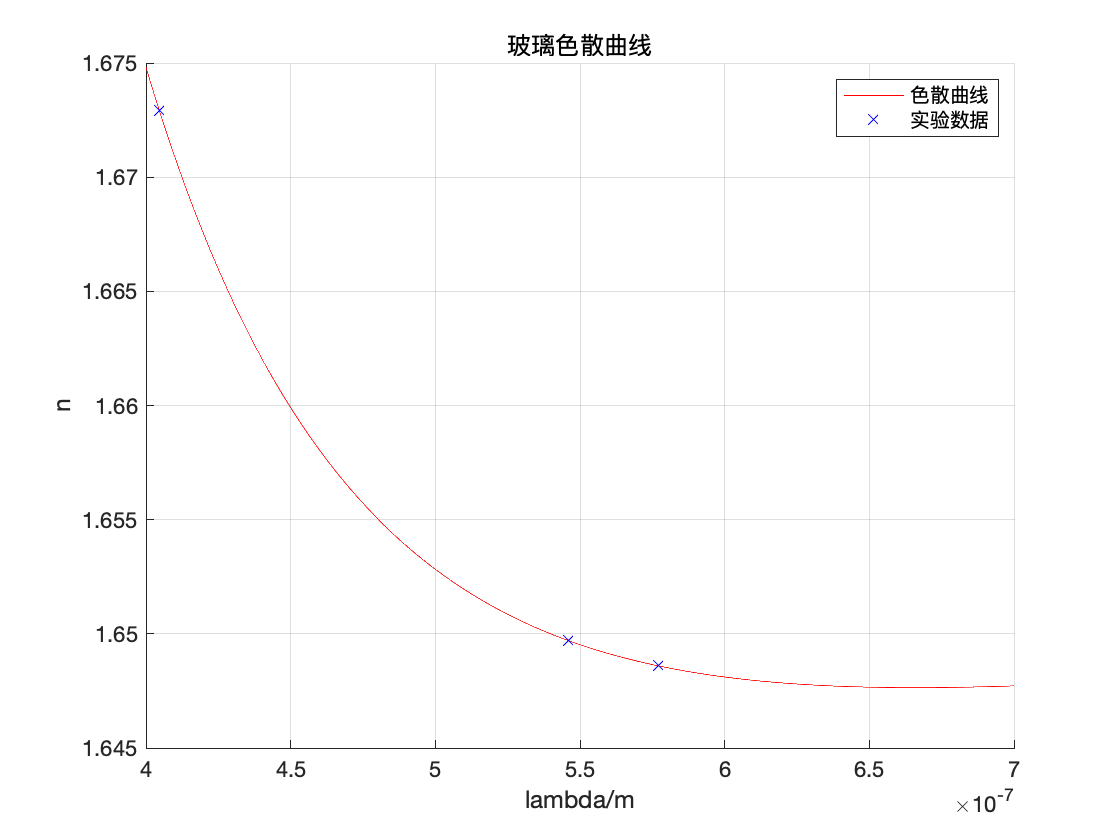
\includegraphics[scale=0.25]{色散曲线.png}
    \caption{\emph{色散曲线}}
\end{figure}

对于注水三棱镜,由表\ref{5}同理计算可得$n_{\text{紫}}^\prime=1.3384$,
$n_{\text{绿}}^\prime=1.3334$,$n_{\text{黄}}^\prime=1.3319$.

\section{思考}
已调好望远镜光轴垂直主轴,若将平面镜取下后,又放到载物台上(放的位置与拿下前的位置不同),发现两镜面又不垂直望远镜光轴了,
是因为再次放上平面镜后平面镜镜面不再垂直于主轴,因此镜面与望远镜也不垂直;这不能说明望远镜光轴还没调好.~
\end{document}